\section{Implementation Methods}
\subsection{Numerical Optimization Methods}
In all but the simplest cases, an analytical solution to (P)
\begin{align*}
    x^*\in \mathrm{arg} \mathrm{min}f(x)\\
    \mathrm{s.t.} x\in\mathbb{Q}
\end{align*}
is said to be convex, if $f: \mathbb{R}^n\rightarrow\mathbb{R} \textrm{and the set} \mathbb{Q}$ are convex.
$\Rightarrow$ Numerical computation of a solution that is ''good enough''
\textbf{iterative optimization methods}
Given an initial guess $x^{(0)}$ produce a sequence of iterates \[x^{(i+1)} = \Psi(x^{(i)},f,\mathbb{Q}), \hspace{3mm} i=0,\dots,m-1\]
such that \[|f(x^{(m)})-f(x^*)| \leq\epsilon \hspace{3mm}\textrm{and}\hspace{3mm} \mathrm{dist}(x^{(m)},\mathbb{Q})\leq \delta\]
where $\epsilon$ and $\delta$ are user defined tolerances.
\subsection{Unconstrained Minimization} \[\underset{x}{\mathrm{min}}f(x) \hspace{3mm} \mathrm{with:} f:\mathbb{R}^n \rightarrow \mathbb{R}\] 
\begin{itemize}
    \item $f$ convex, twice continously differentiable
    \item We assume optimal value $p^* = \underset{x}{\mathrm{min}}f(x)$ is finite
\end{itemize}
\subsubsection{Optimality Conditions:}
Assume $f(\cdot)$ differentiable at $x^*$ if $f$ is convex, then $x^*$ is a global minimizer iff $\nabla f(x^*) = 0$
\subsection{Descent Methods}
Regard the abstract method \[x^{(i+1)} = x^{(i)} + h^{(i)} \Delta x^{(i)}\]
\begin{itemize}
    \item $\Delta x$ is the \textbf{step} or \textbf{search direction}
    \item $h^{(i)}$ is the \textbf{step size} or \textbf{length}
\end{itemize}
we call (M) a \textbf{descent method} if $f(x^{(i+1)}) < f(x^{(i)}$ in particular
\begin{itemize}
    \item if $\nabla f(x^{(i)})^T\Delta x^{(i)},$ then $\Delta x^{(i)}$ is a \textbf{descent direction}
    \item There exists a $h{(i)}> 0$ such that $f(x^{(i+1)}) < f(x^{(i)})$ 
\end{itemize}
\subsubsection{Gradient Method}
\textbf{Idea:} Gradient $\nabla f$ gives direction of steepest local ascent
$\Rightarrow$ Make steps of size $h$ into anti-gradient direction $-\nabla f$
\[\boxed{x^{(i+1)} = x^{(i)} = x^{(i)} - h^{(i)} \nabla f(x^{(i)})}\]
\vfill\null\columnbreak

\subsubsection{Newton's Method}
\textbf{Idea:} Minimize second-order approximation of $f$ at current iterate $x_i:$
\begin{gather*}
     x^{(i+1)} = \mathrm{arg} \underset{x}{\mathrm{min}} f(x^{(i)}) + \nabla f(x^{(i)})^T (x-x^{(i)})\\ + \frac{1}{2}(x-x^{(i)})^T\nabla^2 f(x_i)(x-x^{(i)})\\ \nabla_x (f(x^{(i)}))+\nabla f(x^{(i)})^T(x-x^{(i)}) +\\ 
     \frac{1}{2}(x-x^{(i)})^T\nabla^2 f(x^{(i)})(x-x^{(i)})(x-x^{(i)})|_{x= X^{(i+1)}} = 0\\
     \Leftrightarrow \nabla f(x^{(i)}) +\nabla^2f(x^{(i)})(x^{i+1)}-x^{(i)}) = 0\\
     \Leftrightarrow x^{(i+1)} = x^{(i)}\underbrace{-(\nabla^2f(x^{(i)})^{-1}\nabla f(x^{(i)})}_{\textrm{Newton direction }\Delta x_{nt}}
\end{gather*}
Since $\Tilde{f}$ is not an upper bound on $f$, full Newton step does not necessarily yield descent (i.e. $f(x^{(i+1)}) > f(x^{(i)})$ might occur\\
\textbf{Idea:} use step size $h^{(i)}>0$ such that Newton step yields descent. \\
\textbf{Newton step: }$\boxed{x^{(i+1)} = x^{(i)} - h^{(i)}(\nabla^2f(x^{(i)}) ^{-1}\nabla f(x^{(i)})}$
\subsubsection{Line Search}
\textbf{Newton step:} $\boxed{x^{(i+1)}=x^{(i)}+h^{(i)}\Delta x_{nt} }$\\
\textbf{Problem: } Find $h^{(i)} > 0$ s.t. $f(x^{(i)}+h^{(i)}\Delta x_{nt }) <f(x^{(i)})$
\textbf{Line search methods:}
\begin{itemize}
\item \textbf{Exact:} Compute \textbf{best} $h^{(i)}$
\[h^{(i)*}= \mathrm{arg}\underset{h>0}{\mathrm{min}}f(x^{(i)}+h^{(i)}\Delta x_{nt})\]
optimization in 1 variable $\rightarrow$ solve by bisection time consumin (rquires many evaluations of $f$)
\item \textbf{Inexact} Finds $h^{(i)}$ that decreases $f$ by some amount. Example: \textbf{Backtracking} line search.
\end{itemize}
For $\alpha \in (0,0.5)$ and $\beta \in (0,1)$:\\
\hspace*{3mm} \textbf{Initialize} $h^{(i)} = 1$\\
\hspace*{3mm} \textbf{while} $f(x^{(i)}+h^{(i)}\Delta x_{nt}) > f(x^{(i)})+\alpha h^{(i)}\nabla f(x^{(i)})^T\Delta x_{nt}\\$
\hspace*{5mm}    \textbf{do} $h^{(i)}\leftarrow\beta h^{(i)}$
\subsection{constrained Optimization}
\subsubsection{Equality constr. Newton's Method}
minimize $f(x)$ s.t. $Ax=b$
\begin{gather*}
    \Delta x_{nt}
(x_i) \in \textrm{arg }\underset{\Delta x}{\textrm{min}} \frac{1}{2}\Delta x^T\nabla^2 f(x^{(i)})\Delta x+\nabla f(x^{(i)})\Delta x \\
\textrm{s.t. } A \Delta x = -A x^{(i)} + b\\
\end{gather*}
\begin{align*}
\nabla^2 f(x^{(i)})\Delta x + \nabla f(x^{(i)}) + A^T \lambda &= 0\\
    A\Delta x &= 0\\
    \Updownarrow\\
    \begin{bmatrix}
    \nabla^2f(x^{(i)} & A^T \\
    A & 0
    \end{bmatrix}
    \begin{bmatrix}
    \Delta x \\
    \lambda 
    \end{bmatrix} = \begin{bmatrix}
    -\nabla f(x^{(i)}) \\ 0
    \end{bmatrix}
\end{align*}
\subsubsection{Constrained minimization: gradient method}
minimize $f(x)$ subj. to $x\in Q $ convex L-smooth constraints in gradient step: $x^{(i+1)} = \pi _Q (x^{(i)}- h^{(i)} \nabla f(x^{(i)}), h^{(i)} = \frac{1}{2}$\\
$\pi_Q$ is a projection: \begin{gather*}
    \pi_Q (y) = \textrm{arg} \underset{x}{\textrm{min }} \frac{1}{2}||x-y||_2^2\\
    \textrm{s. t.} x \in \mathcal{Q}
\end{gather*}
\begin{itemize}
    \item numerically (does need to be dualized slower)
    \item projection easy to compute efficient algorithm
\end{itemize}

\subsection{constrainted minimization: interior Point methods}
min $f(x)$ subj. to. $g_i(x) \leq 0$
\begin{itemize}
    \item $f(x^*)$ finite \& attained feasible set closed \& compact
    \item $f,g_i$ convex, twice diff.
    \item strrict feasibility
\end{itemize}
$\Rightarrow $ reformulate problem as unconstrained problem \\
auxiliary funct: $\hat{f}(x) := f(x) + K \phi (x)$ s.t $\hat{f}(x) = \infty$ if constr. violated.\\
Indicator funct: $\phi (x) = \sum^m_{i=1}I(g_i)(x)), K=1$ where $I (u) = 0 if u \leq 0, \infty else$
\vfill\null\columnbreak
\subsubsection{Barrier Interior-point method}
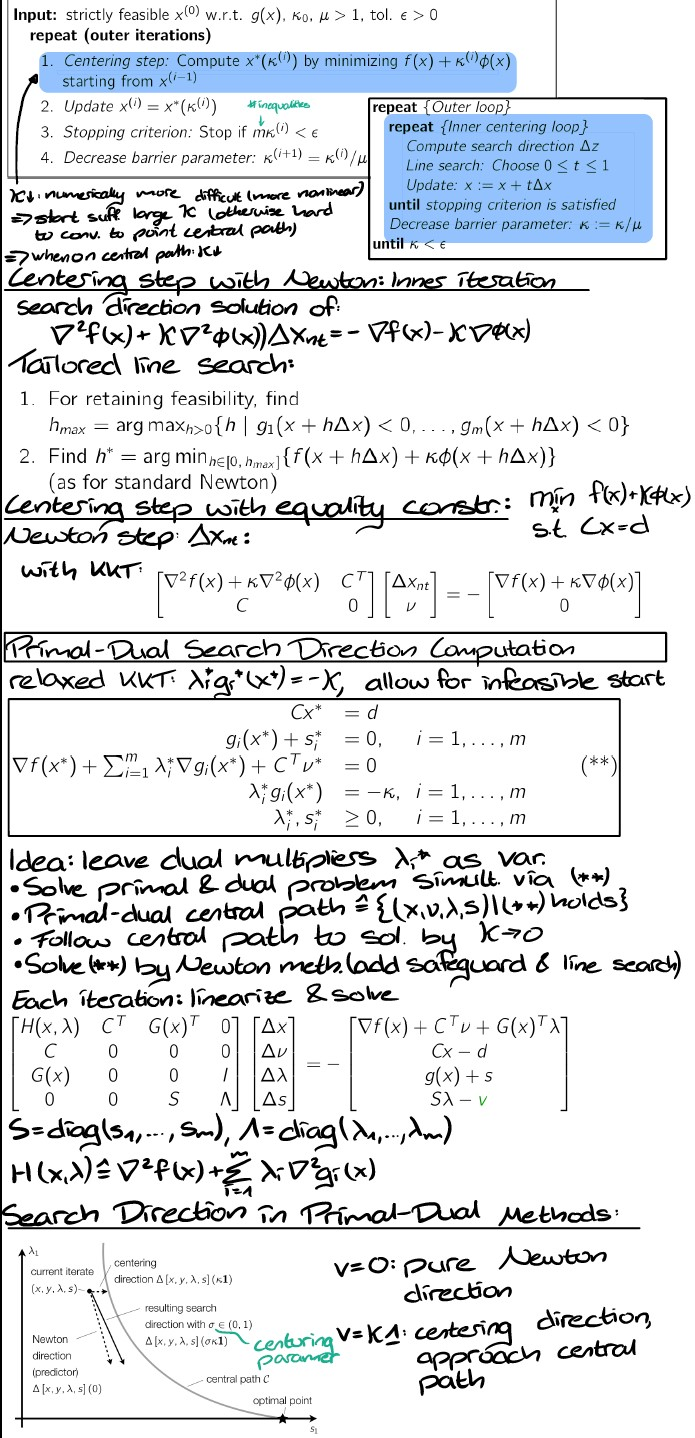
\includegraphics[width= 0.99\linewidth]{MPC_summary/Images/mag_num.jpg}